
\documentclass[nooutcomes]{ximera}
%\documentclass[space,handout,nooutcomes]{ximera}

% For preamble materials

\usepackage{pgf,tikz}
\usepackage{mathrsfs}
\usetikzlibrary{arrows}
\usepackage{framed}
\usepackage{amsmath}
%\pgfplotsset{compat=1.16}

\graphicspath{
  {./}
  {algorithms/}
  {../algorithms/}
}

\pdfOnly{\renewenvironment{image}[1][]{\begin{center}}{\end{center}}}

%%% This set of code is all of our user defined commands
\newcommand{\bysame}{\mbox{\rule{3em}{.4pt}}\,}
\newcommand{\N}{\mathbb N}
\newcommand{\C}{\mathbb C}
\newcommand{\W}{\mathbb W}
\newcommand{\Z}{\mathbb Z}
\newcommand{\Q}{\mathbb Q}
\newcommand{\R}{\mathbb R}
\newcommand{\A}{\mathbb A}
\newcommand{\D}{\mathcal D}
\newcommand{\F}{\mathcal F}
\newcommand{\ph}{\varphi}
\newcommand{\ep}{\varepsilon}
\newcommand{\aph}{\alpha}
\newcommand{\QM}{\begin{center}{\huge\textbf{?}}\end{center}}

\renewcommand{\le}{\leqslant}
\renewcommand{\ge}{\geqslant}
\renewcommand{\a}{\wedge}
\renewcommand{\v}{\vee}
\renewcommand{\l}{\ell}
\newcommand{\mat}{\mathsf}
\renewcommand{\vec}{\mathbf}
\renewcommand{\subset}{\subseteq}
\renewcommand{\supset}{\supseteq}
\renewcommand{\emptyset}{\varnothing}
\newcommand{\xto}{\xrightarrow}
\renewcommand{\qedsymbol}{$\blacksquare$}
\newcommand{\bibname}{References and Further Reading}
\renewcommand{\bar}{\protect\overline}
\renewcommand{\hat}{\protect\widehat}
\renewcommand{\tilde}{\widetilde}
\newcommand{\tri}{\triangle}
\newcommand{\minipad}{\vspace{1ex}}
\newcommand{\leftexp}[2]{{\vphantom{#2}}^{#1}{#2}}

%% More user defined commands
\renewcommand{\epsilon}{\varepsilon}
\renewcommand{\theta}{\vartheta} %% only for kmath
\renewcommand{\l}{\ell}
\renewcommand{\d}{\, d}
\newcommand{\ddx}{\frac{d}{dx}}
\newcommand{\dydx}{\frac{dy}{dx}}


\usepackage{bigstrut}


\newenvironment{sectionOutcomes}{}{}

\usepackage{array}
%\setlength{\extrarowheight}{-.2cm}   % Commented out by Findell to fix table headings.  Was this for typesetting division?  
\newdimen\digitwidth
\settowidth\digitwidth{9}
\def~{\hspace{\digitwidth}}
\def\divrule#1#2{
\noalign{\moveright#1\digitwidth
\vbox{\hrule width#2\digitwidth}}}


\title{Ratios}
\author{Bart Snapp and Brad Findell and Jenny Sheldon}
\begin{document}
\begin{abstract}
Problems about ratios.
\end{abstract}
\maketitle


%\begin{problem}
%Problem
%\begin{freeResponse}
%\begin{hint}
%Hint
%\end{hint}
%\end{freeResponse}
%\end{problem} 






\begin{problem}
A certain punch is made by mixing $4$ cups of fruit juice with $5$ cups of sparkling water.  Fill in the table below to find how many cups of fruit juice you will need to mix with $19$ cups of sparkling water to get a punch in the same recipe.

\[
\begin{array}{|l|c|c|c|} \hline
\textrm{fruit juice} & 4 & \answer[given]{\frac{4}{5}} & \answer[given]{\frac{76}{5}} \\ \hline
\textrm{sparkling water} &5 & 1 & 19 \\ \hline \hline
\textrm{punch} & 9 & \answer[given]{1.8} & \answer[given]{34.2} \\ \hline
\end{array}
\]
\end{problem}


\begin{problem}
A contractor usually mixes $8$ kilograms of sand with $11$ kilograms of rocks to make a parking area for equipment.  How many kilograms of sand should the contractor mix with $20$ kilograms of rocks in order to make the same mixture, but for a larger parking area?  Fill out the table below to answer this question.

\[
\begin{array}{|l|c|c|c|c|} \hline
\textrm{sand} & 8 & 16 & 4 & 20 \\ \hline
\textrm{rocks} & 11 & \answer[given]{22} & \answer[given]{5.5} & \answer[given]{27.5} \\ \hline \hline
\textrm{mixture} & 19 & \answer[given]{38} & \answer[given]{9.5} & \answer[given]{47.5} \\ \hline
\end{array}
\]
\end{problem}





\begin{problem}
Jenny mixes $\frac{5}{7}$ of a cup of water with $\frac{1}{2}$ of a cup of insect repellent concentrate to spray around her yard.  How much water and insect repellent will Jenny need in order to make $3$ cups of this mixture?  Fill out the table below to answer this question.

\[
\begin{array}{|l|c|c|c|c|} \hline
\textrm{water} & \frac{5}{7} & 10 & \answer[given]{\frac{10}{17}} & \answer[given]{\frac{30}{17}} \\ \hline
\textrm{concentrate}& \frac{1}{2} & \answer[given]{7} & \answer[given]{\frac{7}{17}} & \answer[given]{\frac{21}{17}} \\ \hline \hline
\textrm{mixture} & & \answer[given]{17} & 1 & 3 \\ \hline
\end{array}
\]

\end{problem}




\begin{problem}
A bike is traveling at a constant rate of $4$ miles every $15$ minutes.  How far does the bike travel in $35$ minutes?  We will use the double number line below to answer this question.

\begin{center}
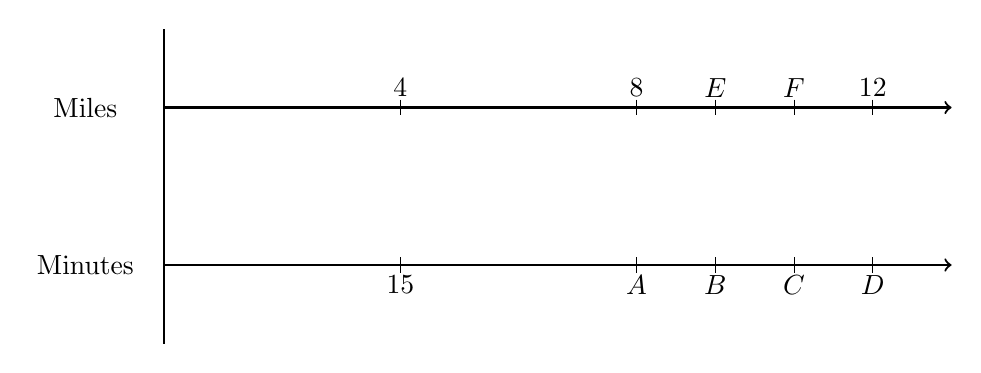
\begin{tikzpicture}
\draw[thick] (0,-2)--(0,2);
\draw[->, thick] (0,1)--(10,1);
\draw[->, thick] (0, -1) -- (10, -1);
\node at (-1, 1) {Miles};
\node at (-1, -1) {Minutes};
\node at (3, -1.25) {$15$};
\node at (3, 1.25) {$4$};
\node at (6, -1.25) {$A$};
\node at (6, 1.25) {$8$};
\node at (7, -1.25) {$B$};
\node at (7, 1.25) {$E$};
\node at (8, -1.25) {$C$};
\node at (8, 1.25) {$F$};
\node at (9, -1.25) {$D$};
\node at (9, 1.25) {$12$};
\foreach \x in {3, 6, 7, 8, 9} \draw (\x, -1.1)--(\x, -0.9); 
\foreach \y in {3, 6, 7, 8, 9} \draw (\y, 1.1)--(\y, 0.9);

\end{tikzpicture}
\end{center}
\begin{enumerate}
	\item What is the value we should mark on the line at point $A$? $\answer[given]{30}$
	\item What is the value we should mark on the line at point $D$? $\answer[given]{45}$
	\item Which point on the line corresponds to $35$ minutes?
		 \begin{multipleChoice}
		 	\choice[correct]{$B$}
			\choice{$C$}
			\choice{$E$}
			\choice{$F$}
		 \end{multipleChoice}
	\item How far did the bike travel in $35$ minutes? $\answer[given]{8+\frac{4}{3}}$ miles
\end{enumerate}

\end{problem}



\begin{problem}
If $350$ yards of yarn weighs $210$ grams, how much does $530$ yards of the same yarn weigh?  Fill in the missing values on the double number line below, and then solve the problem.

\begin{center}
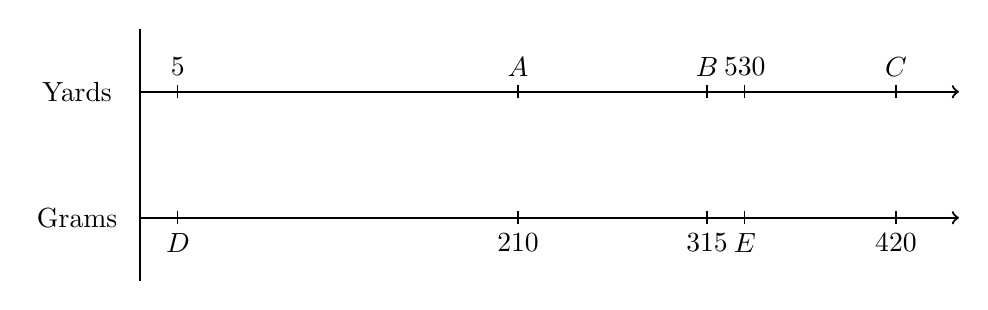
\begin{tikzpicture}[scale=0.8]
\draw[thick] (0,-2)--(0,2);
\draw[->, thick] (0,1)--(13,1);
\draw[->, thick] (0, -1) -- (13, -1);
\node at (-1, 1) {Yards};
\node at (-1, -1) {Grams};
\node at (0.6, -1.4) {$D$};
\node at (0.6, 1.4) {$5$};
\node at (6, -1.4) {$210$};
\node at (6, 1.4) {$A$};
\node at (9, -1.4) {$315$};
\node at (9, 1.4) {$B$};
\node at (9.6, -1.4) {$E$};
\node at (9.6, 1.4) {$530$};
\node at (12, -1.4) {$420$};
\node at (12, 1.4) {$C$};
\foreach \x in {0.6, 6, 9, 9.6, 12} \draw (\x, -1.1)--(\x, -0.9); 
\foreach \y in {0.6, 6, 9, 9.6, 12} \draw (\y, 1.1)--(\y, 0.9);
\end{tikzpicture}
\end{center}

\begin{prompt}	
	We have $A = \answer[given]{350}$, $B = \answer[given]{525}$, and $C = \answer[given]{700}$.
	
	We also have $D = \answer[given]{3}$, and $E = \answer[given]{318}$.
	
	Finally, $530$ yards of the yarn weighs $\answer[given]{318}$ grams.
\end{prompt}
\end{problem}



\begin{problem}
We mix red and blue paint in a $2 : 4$ ratio to make a lovely shade of violet paint.  How many liters of each paint do we need to make $21$ liters of paint total? 

Suzi solves the above problem using the following picture.

\begin{center}
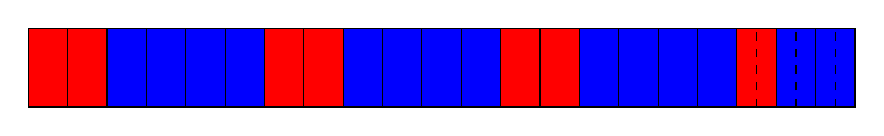
\begin{tikzpicture}
\draw[fill=red] (0,0)--(1,0)--(1,1)--(0,1)--(0,0);
\draw[fill=blue] (1,0)--(3,0)--(3,1)--(1,1)--(1,0);
\draw[fill=red] (3,0)--(4,0)--(4,1)--(3,1)--(3,0);
\draw[fill=blue](4,0)--(6,0)--(6,1)--(4,1)--(4,0);
\draw[fill=red] (6,0)--(7,0)--(7,1)--(6,1)--(6,0);
\draw[fill=blue] (7,0)--(9,0)--(9,1)--(7,1)--(7,0);
\draw[fill=red] (9,0)--(9.5,0)--(9.5,1)--(9,1)--(9,0);
\draw[fill=blue] (9.5,0)--(10.5,0)--(10.5,1)--(9.5,1)--(9.5,0);
\foreach \x in {0.5, 1, 1.5, ..., 10} \draw (\x,0)--(\x, 1);
\draw[dashed] (9.25,0)--(9.25,1);
\draw[dashed] (9.75,0)--(9.75,1);
\draw[dashed] (10.25, 0)--(10.25,1);
\end{tikzpicture}
\end{center}

\begin{enumerate}
\item Explain what Suzi has drawn, and how it relates to the problem.
\begin{freeResponse}
\begin{hint}
Suzi has drawn the 21 liters of paint to be made, one box for each liter.  She then colors the boxes in the pattern $2$ red, $4$ blue, until she has fewer than 6 boxes remaining.  At the end, she splits up the remaining boxes into six equal parts so that she can color two of the remaining parts red, and four blue.
\end{hint}
\end{freeResponse}
\item Use Suzi's picture to answer the original question.
\begin{prompt}
We should use $\answer[given]{7}$ liters of red paint and $\answer[given]{14}$ liters of blue paint.
\end{prompt}
\end{enumerate}

\end{problem}




\begin{problem}
We mix red and blue paint in a $2 : 4$ ratio to make a lovely shade of violet paint.  How many liters of each paint do we need to make $21$ liters of paint total? 

Marc solves the above problem using the following picture.

\begin{center}
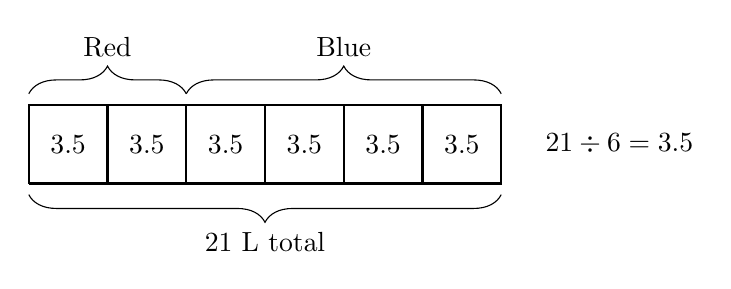
\begin{tikzpicture}
\draw[thick] (0,0)--(6,0)--(6,1)--(0,1)--(0,0);
\foreach \x in {1, 2, ..., 5} \draw[thick] (\x, 0) -- (\x, 1);
\draw [decorate,decoration={brace,amplitude=10pt,mirror},xshift=0pt,yshift=-4pt]
            (0,0) -- (6,0) node [black,midway,yshift=-0.6cm] {$21$ L total};
\draw [decorate,decoration={brace,amplitude=10pt},xshift=0pt,yshift=4pt]
            (0,1) -- (2,1) node [black,midway,yshift=0.6cm] {Red};
\draw [decorate,decoration={brace,amplitude=10pt},xshift=0pt,yshift=4pt]
            (2,1) -- (6,1) node [black,midway,yshift=0.6cm] {Blue};
\node at (7.5, 0.5) {$21 \div 6 = 3.5$};
\foreach \y in {0.5, 1.5, 2.5, 3.5, 4.5, 5.5} \node at (\y, 0.5) {$3.5$};
\end{tikzpicture}
\end{center}

\begin{enumerate}
\item Explain what Marc has drawn, and how it relates to the problem.
\begin{freeResponse}
\begin{hint}
Marc has drawn the $6$ parts of the ratio, and labeled the two parts red and four parts blue.  He then figures out how to split up the $21$ liters across the $6$ boxes, and sees that we should put $3.5$ liters in each part.
\end{hint}
\end{freeResponse}
\item Use Marc's picture to answer the original question.
\begin{prompt}
We should use $\answer[given]{7}$ liters of red paint and $\answer[given]{14}$ liters of blue paint.
\end{prompt}
\end{enumerate}

\end{problem}





\begin{problem}
We mix $5$ parts iced tea with $2$ parts lemonade to make a refreshing summer beverage.  How much lemonade should we mix with $1.5$ cups of iced tea to make just one serving of this refreshing beverage?  Use a method similar to Marc's method of the previous problem to answer this question.

\begin{center}
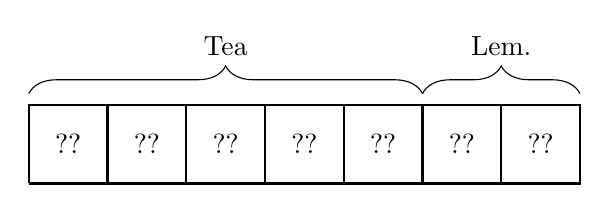
\begin{tikzpicture}
\draw[thick] (0,0)--(7,0)--(7,1)--(0,1)--(0,0);
\foreach \x in {1, 2, ..., 6} \draw[thick] (\x, 0) -- (\x, 1);
\draw [decorate,decoration={brace,amplitude=10pt},xshift=0pt,yshift=4pt]
            (0,1) -- (5,1) node [black,midway,yshift=0.6cm] {Tea};
\draw [decorate,decoration={brace,amplitude=10pt},xshift=0pt,yshift=4pt]
            (5,1) -- (7,1) node [black,midway,yshift=0.6cm] {Lem.};
\foreach \y in {0.5, 1.5, 2.5, 3.5, 4.5, 5.5, 6.5} \node at (\y, 0.5) {$??$};
\end{tikzpicture}

\begin{enumerate}
\item What value should go in each box in this case? $\answer[given]{0.3}$ cups
\item How much lemonade should we mix with $1.5$ cups of iced tea? $\answer[given]{0.6}$ cups
\end{enumerate}
\end{center}



\end{problem}











\begin{problem}
A certain shade of green paint is made by mixing $5$ parts of yellow paint with $9$ parts of blue paint.  How many parts of yellow paint would you need to mix with $1$ part blue paint?  For fun, try to use a new method to solve this problem!

\begin{prompt}
You would use $\answer[given]{\frac{5}{9}}$ parts yellow paint.
\end{prompt}
\end{problem}


\begin{problem}
A certain shade of green paint is made by mixing $12$ parts of yellow paint with $4$ parts of blue paint.  How many parts of blue paint would you need to mix with $1$ part yellow paint?  For fun, try to use a new method to solve this problem!

\begin{prompt}
You would use $\answer[given]{\frac{4}{12}}$ parts blue paint.
\end{prompt}
\end{problem}



\begin{problem}
Two kayakers are traveling at a constant speed.  Doug travels $300$ meters in $8$ minutes, while Phil travels $350$ meters in $9$ minutes.  Who is traveling faster?

\begin{multipleChoice}
	\choice[correct]{Phil travels faster, because he covers about $39$ meters per minute.}
	\choice{Doug travels faster, because he covers about $38$ meters per minute.}
	\choice{Phil travels faster, because he travels farther.}
	\choice{Doug travels faster, because he travels for fewer minutes.}
\end{multipleChoice}
\end{problem}


\begin{problem}
Vi is making biscuits.  Her recipe calls for $2 \frac{3}{4}$ teaspoons of baking powder and $2 \frac{1}{3}$ cups of flour.  She got a bit mixed up and instead added $3 \frac{2}{4}$ teaspoons of baking powder to her bowl with $2 \frac{1}{3}$ cups of flour.  How much more flour should she add to the bowl in order to still be using the same recipe?

\begin{prompt}
 Vi should add $\answer[given]{\frac{7}{11}}$ of a cup of flour to the bowl.
\end{prompt}
\end{problem}



\begin{problem}
Three snails are moving at a constant rate.

\begin{itemize}
	\item Snail $A$ travels $0$ inches in $4$ minutes.
	\item Snail $B$ travels $4$ inches in $0$ minutes.
	\item Snail $C$ travels $0$ inches in $0$ minutes.
\end{itemize}

How fast does each snail travel one inch?  Select all correct answers below.
\begin{selectAll}
	\choice[correct]{Snail $A$ travels $0$ inches in $1$ minute.}
	\choice{Snail $B$ travels $4$ inches in $1$ minute.}
	\choice{Snail $C$ travels $0$ inches in $1$ minute.}
	\choice{We do not know how far Snail $A$ travels in $1$ minute.}
	\choice{Snail $A$'s information is impossible.}
	\choice[correct]{Snail $B$'s information is impossible.}
	\choice{Snail $C$'s information is impossible.}
	\choice{We do not know how far Snail $A$ travels in $1$ minute.}
	\choice{We do not know how far Snail $B$ travels in $1$ minute.}
	\choice[correct]{We do not know how far Snail $C$ travels in $1$ minute.}
\end{selectAll}

\begin{problem}
We have different issues finding the distances traveled by two of the snails in one minute.  Explain how the two problems are different.
\begin{freeResponse}
	\begin{hint}
	With Snail $B$, the snail is not using any time to cover the distance.  In this case, we have an impossible situation: movement without using time.  With Snail $C$, however, as no time elapses, the snail does not move.  This could mean essentially anything - after 1 minute, the snail could have moved essentially any distance.  We do not have enough information to answer this question!
	\end{hint}
\end{freeResponse}
\end{problem}
\end{problem}



\begin{problem}
How is the previous problem related to division with zero?
\begin{freeResponse}
	One way to solve the problem is to find the rate at which the snails move.  In order to find this rate, we divide the distance by the number of minutes.  Snail $A$'s speed is $0 \div 4$ inches per minute, Snail $B$'s rate is $4 \div 0$ inches per minute (which is undefined), and Snail $C$'s rate is $0 \div 0$ inches per minute.  Look again at the previous problem and think about what you know about $4 \div 0$ versus $0 \div 0$!
\end{freeResponse}
\end{problem}




\end{document}



